% On découpe ce document complexe en plusieurs sous-fichiers séparés.
% Cela permettra notamment de réarranger les transparents facilement 
% lors de l'élaboration du document.

% La définition de la classe beamer avec tous les styles afférents

\RequirePackage{currfile} 

\documentclass{beamer}

%%%%%%%%%%%%%%%%%%%%%%%%%%%%%%%%%%%%%%%%%
% Beamer Presentation
% LaTeX Template
% Version 1.0 (10/11/12)
%
% This template has been downloaded from:
% http://www.LaTeXTemplates.com
%
% License:
% CC BY-NC-SA 3.0 (http://creativecommons.org/licenses/by-nc-sa/3.0/)
%
%%%%%%%%%%%%%%%%%%%%%%%%%%%%%%%%%%%%%%%%%

%----------------------------------------------------------------------------------------
%	PACKAGES AND THEMES
%----------------------------------------------------------------------------------------




\mode<presentation> {

% The Beamer class comes with a number of default slide themes
% which change the colors and layouts of slides. Below this is a list
% of all the themes, uncomment each in turn to see what they look like.

%\usetheme{default}
%\usetheme{AnnArbor}
%\usetheme{Antibes}
%\usetheme{Bergen}
%\usetheme{Berkeley}
%\usetheme{Berlin}
%\usetheme{Boadilla}
%\usetheme{CambridgeUS}
%\usetheme{Copenhagen}
%\usetheme{Darmstadt}
%\usetheme{Dresden}
%\usetheme{Frankfurt}
%\usetheme{Goettingen}
%\usetheme{Hannover}
%\usetheme{Ilmenau}
%\usetheme{JuanLesPins}
%\usetheme{Luebeck}
%\usetheme{Madrid}		
%\usetheme{Malmoe}
%\usetheme{Marburg}
%\usetheme{Montpellier}
%\usetheme{PaloAlto}
%\usetheme{Pittsburgh}
%\usetheme{Rochester}
%\usetheme{Singapore}
%\usetheme{Szeged}
\usetheme{Warsaw}

% As well as themes, the Beamer class has a number of color themes
% for any slide theme. Uncomment each of these in turn to see how it
% changes the colors of your current slide theme.

%\usecolortheme{albatross}
%\usecolortheme{beaver}
%\usecolortheme{beetle}
%\usecolortheme{crane}
%\usecolortheme{dolphin}
%\usecolortheme{dove}
%\usecolortheme{fly}
%\usecolortheme{lily}
%\usecolortheme{orchid}
%\usecolortheme{rose}
%\usecolortheme{seagull}
%\usecolortheme{seahorse}
\usecolortheme{whale}
%\usecolortheme{wolverine}

%\setbeamertemplate{footline} % To remove the footer line in all slides uncomment this line
%\setbeamertemplate{footline}[frame number] % To replace the footer line in all slides with a simple slide count uncomment this line

%\setbeamertemplate{navigation symbols}{} % To remove the navigation symbols from the bottom of all slides uncomment this line

\setbeamercovered{transparent} % Fait apparaître les animations en grisé (utile pour la conception, mais peut être commenté lors de la remise du document final)

% Pour utiliser une police à empattements partout
\usefonttheme{serif}

% Pour rajouter la numérotation des frames dans les pieds de page
\newcommand*\oldmacro{}%
\let\oldmacro\insertshorttitle%
\renewcommand*\insertshorttitle{%
  \oldmacro\hfill%
  \insertframenumber\,/\,\inserttotalframenumber}

}

\usepackage{graphicx} % Allows including images
\usepackage{booktabs} % Allows the use of \toprule, \midrule and \bottomrule in tables




% Les autres packages utiles  notamment pour le français, les accents ou Python
\usepackage{natbib}         % Pour la bibliographie
\usepackage{url}            % Pour citer les adresses web
\usepackage[T1]{fontenc}    % Encodage des accents
\usepackage[utf8]{inputenc} % Lui aussi
\usepackage[frenchb]{babel} % Pour la traduction française
\usepackage{numprint}       % Histoire que les chiffres soient bien

\usepackage{amsmath}        % La base pour les maths
\usepackage{mathrsfs}       % Quelques symboles supplémentaires
\usepackage{amssymb}        % encore des symboles.
\usepackage{amsfonts}       % Des fontes, eg pour \mathbb.

\usepackage{cancel}

%\usepackage[svgnames]{xcolor} % De la couleur

%%% Si jamais vous voulez changer de police: décommentez les trois 
%\usepackage{tgpagella}
%\usepackage{tgadventor}
%\usepackage{inconsolata}

%%% Pour L'utilisation de Python
\usepackage{minted}
\usemintedstyle{friendly}

\usepackage{graphicx} % inclusion des graphiques
\usepackage{wrapfig}  % Dessins dans le texte.

\usepackage{tikz}     % Un package pour les dessins (utilisé pour l'environnement {code})
\usepackage[framemethod=TikZ]{mdframed}

% Les macros et raccourcis personnels
% Ce fichier contient toutes les macros que vous pouvez avoir envie de définir 
% si vous les utilisez plusieurs fois dans le document.

\PassOptionsToPackage{svgnames}{color}

% Un environnement pour bien présenter le code informatique
\newenvironment{code}{%
\begin{mdframed}[linecolor=green,innerrightmargin=30pt,innerleftmargin=30pt,
backgroundcolor=black!5,
skipabove=10pt,skipbelow=10pt,roundcorner=5pt,
splitbottomskip=6pt,splittopskip=12pt]
}{%
\end{mdframed}
}

% Un raccourci pour composer les unités correctement (en droit)
% Exemple: $v = 10\U{m.s^{-1}}$
\newcommand{\U}[1]{~\mathrm{#1}}

% Les guillemets \ofg{par exemple}
\newcommand{\ofg}[1]{\og{}#1\fg{}}

% Le d des dérivées doit être droit: \frac{\dd x}{\dd t}
\newcommand{\dd}{\text{d}}

% La dérivée temporelle, tellement courante en physique, avec les d droits
\newcommand{\ddt}[1]{\frac{\dd #1}{\dd t}}

% Des parenthèses, crochets et accolades qui s'adaptent automatiquement à la 
% taille de ce qu'il y a dedans
\newcommand{\pa}[1]{\left(#1\right)}
\newcommand{\pac}[1]{\left[#1\right]}
\newcommand{\paa}[1]{\left\{#1\right\}}

% Un raccourci pour écrire une constante
\newcommand{\cte}{\text{C}^{\text{te}}}

% Pour faire des indices en mode texte (comme les énergie potentielles)
\newcommand{\e}[1]{_{\text{#1}}}

% Le produit vectoriel a un nom bizarre:
\newcommand{\vectoriel}{\wedge}


% On définit le titre et l'auteur du document

% L'argument optionnel (entre crochets) donne le titre qui sera mis sur chaque slide
\title[TIPE Mercure]{TIPE: Précession du Périhélie de Mercure}
\author{Jean-Julien \textsc{Fleck}} % Votre nom
% L'épreuve b(car on n'a pas le droit de signaler sa provenance à un concours) (là encore, l'argument optionnel apparaît sur chaque slide)
\institute()[TIPE]{Épreuve de TIPE}
\date{Session 2019} 

% On démarre le document proprement dit
\begin{document}

% La page de titre et la table des matières
% Rien d'autre à faire qu'afficher le titre
\begin{frame}
\titlepage 
\end{frame}


% La table des matières utilise ce que vous donnez aux commandes \section et 
% \subsection tout au long de la présentation.
\begin{frame}
\frametitle{Plan de l'exposé} 
\tableofcontents 
\end{frame}


% La première grande partie: introduction du sujet
% Titre de la premiere partie
\section{Introduction Historique}

%%%%%%%%%%%%%%%%%%%%%%%%%%%%%%%%%%%%%%%%%%%%%%%%
% Première diapo
%%%%%%%%%%%%%%%%%%%%%%%%%%%%%%%%%%%%%%%%%%%%%%%%
\begin{frame}
\frametitle{Introduction historique}
\framesubtitle{Position du problème}

\begin{itemize}
	\item	<1->	La mécanique newtonienne, une mécanique bien huilée
	\item	<2->	Précession du périhélie de Mercure
	
	\visible<3->{
	\begin{figure}
	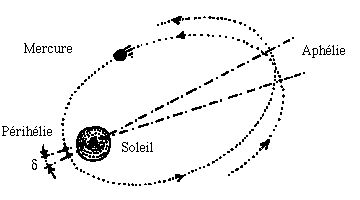
\includegraphics[width=0.8\linewidth]{figures/Fig01}
	\end{figure}
	}
	
\end{itemize}

\end{frame}


%%%%%%%%%%%%%%%%%%%%%%%%%%%%%%%%%%%%%%%%%%%%%%%%
% Deuxième diapo
%%%%%%%%%%%%%%%%%%%%%%%%%%%%%%%%%%%%%%%%%%%%%%%%
\begin{frame}
\frametitle{Introduction historique}
\framesubtitle{Explication classique}

\begin{itemize}
	\item	<1->	Théorie des perturbations: explication de $531''$ d'arc/siècle
	\item	<2->	Vulcain, un bon candidat (Le Verrier, 1859)
	\item	<3->	mais pas de confirmation expérimentale...
	
\end{itemize}

\end{frame}


%%%%%%%%%%%%%%%%%%%%%%%%%%%%%%%%%%%%%%%%%%%%%%%%
% Troisième diapo
%%%%%%%%%%%%%%%%%%%%%%%%%%%%%%%%%%%%%%%%%%%%%%%%
\begin{frame}
\frametitle{Introduction historique}
\framesubtitle{Complément relativiste}

\begin{itemize}
	\item	<1->	La relativité restreinte permet déjà un mieux ($7''$ d'arc 
	en plus par siècle)

	\item	<2->	mais c'est la générale qui va sauver la mise en ajoutant 
	les $43''$ qui manquaient
	
\end{itemize}

\end{frame}


% La 2e partie: Le point de vue de la relativité restreinte
% Titre de la partie
\section{Le point de vue de la Relativité Restreinte}

%%%%%%%%%%%%%%%%%%%%%%%%%%%%%%%%%%%%%%%%%%%%%%%%
% Première diapo (avec des équations)
%%%%%%%%%%%%%%%%%%%%%%%%%%%%%%%%%%%%%%%%%%%%%%%%
\begin{frame}
\frametitle{Relativité Restreinte}
\framesubtitle{Dynamique relativiste}

\begin{itemize}
	\item	<1->	Nouvelle définition de la quantité de mouvement
	
	\onslide <2->{
	$$\vec{p} = \gamma\,m\vec{v}
	\qquad\text{avec}\qquad
	\gamma = \frac{1}{\sqrt{1 - \frac{v^2}{c^2}}}
	$$
	}
	
	\item	<3->	Avec les développements \ofg{classiques} et en posant 
	$u=1/r$, on en arrive à l'équation
	
	\onslide <4->{
	$$
	\onslide <5->
	\underbrace{
	\onslide <4->
	    \frac{\dd^2 u}{\dd \theta^2} + u = \frac{G M m\, E}{L^2\, c^2}
	\onslide <5->
	    }_{
	    \text{Partie usuelle}}
	\onslide <4->
	            + 
	\onslide <6->
	\underbrace{
	\onslide <4->	
	            \frac{\pa{G M m}^2}{L^2\, c^2}\, u
    \onslide <6->
               }_{\text{Partie relativiste}}
	$$
	}
	
	
\end{itemize}

\end{frame}


%%%%%%%%%%%%%%%%%%%%%%%%%%%%%%%%%%%%%%%%%%%%%%%%
% Deuxième diapo
%%%%%%%%%%%%%%%%%%%%%%%%%%%%%%%%%%%%%%%%%%%%%%%%
\begin{frame}
\frametitle{Relativité Restreinte}
\framesubtitle{Équation de l'ellipse}

\begin{itemize}
	\item	<1->	Équation différentielle remise en forme
	
	\onslide <2->{
	$$
	    \frac{\dd u}{\dd \theta} + B^2\, u = A 
	\onslide <3->
	        \quad \text{avec} \quad 
	            B  = \sqrt{1 - \pa{\frac{G M m}{L\, c}}^{\!\!2} }
	$$
	}
	
	\item	<4->	Équation de l'\ofg{ellipse}
	
	\onslide <5->
	$$
	u = \frac{A}{B^2} \pa{1 + e\cos{\pac{B\pa{\theta - \theta_0}}}}
	\onslide <6->
	\quad\text{soit}\quad
	r = \frac{p}{1+e\cos{\pac{B\pa{\theta - \theta_0}}}}
	$$
	
\end{itemize}

\end{frame}

%%%%%%%%%%%%%%%%%%%%%%%%%%%%%%%%%%%%%%%%%%%%%%%%
% Troisième diapo
%%%%%%%%%%%%%%%%%%%%%%%%%%%%%%%%%%%%%%%%%%%%%%%%
\begin{frame}
\frametitle{Relativité Restreinte}
\framesubtitle{Avance du périhélie}

\begin{itemize}
	\item	<1->	L'\ofg{ellipse} ne se referme pas sur elle-même du fait que $B\neq1$
	\item	<2->	Entre deux périhélies successifs, $\theta$ tourne de $2\pi +\delta$ où
	\onslide<3->
	$$
	\boxed{
    \delta = 2\pi\pa{\frac{1}{B} - 1}
    \approx \pi \pa{\frac{G\, M\, m}{L\, c}}^{\!\!2} 
    = \pi \, \frac{G M}{p\, c^2}
    = \pi\, \frac{G M}{a\, c^2\, \pa{1-e^2}}	
    }
	$$
	
	\item	<4-> Malheureusement, l'application numérique ne donne \ofg{que} 
	$7''$ d'arc par siècle...
	
\end{itemize}

\end{frame}


% La 3e partie: Le point de vue de la relativité générale
% Le titre de la partie
\section{Le point de vue de la Relativité Générale}

%%%%%%%%%%%%%%%%%%%%%%%%%%%%%%%%%%%%%%%%%%%%%%%%
% Première diapo
%%%%%%%%%%%%%%%%%%%%%%%%%%%%%%%%%%%%%%%%%%%%%%%%

\begin{frame}
\frametitle{Relativité Générale}
\framesubtitle{Et zut...}

\begin{itemize}
	\item	<1->	Il n'y a plus guère de temps pour parler
	\item	<2->	Alors zou, on balance le résultat des calculs

$$
    \onslide<3->
    \underbrace{
    \onslide<2->    
    \frac{\dd^2 u}{\dd \theta^2} + u 
        = 
        \frac{G M m^2}{L^2} 
    \onslide<3->
    }_{\text{Partie classique}}
    \onslide<2->
    + 
    \onslide<3->
    \underbrace{
    \onslide<2->    
    \frac{3\, G M}{c^2}\, u^2
    \onslide<3->
    }_{\text{RG}}
    \onslide<2->
$$

	\item	<4->	Après avoir bien bossé, on obtient finalement
\onslide<4->
$$
	\boxed{
		\delta = 6\, \pi \, \frac{G M}{a\, c^2\pa{1-e^2}}
			}
$$

\end{itemize}

\end{frame}


%%%%%%%%%%%%%%%%%%%%%%%%%%%%%%%%%%%%%%%%%%%%%%%%
% Deuxième diapo: le code informatique impose un 
% environnement "fragile" pour la frame
%%%%%%%%%%%%%%%%%%%%%%%%%%%%%%%%%%%%%%%%%%%%%%%%

\begin{frame}[fragile]
\frametitle{Relativité Générale}
\framesubtitle{Le code informatique}

\begin{code}
\begin{minted}[linenos]{python}

import scipy as sp
import scipy.optimize

def ma_fonction(x):
    return []

# À vous de remplir les choses adéquates...

\end{minted}
\end{code}
\end{frame}


% Conclusion
% Le titre de la partie
\section{Conclusion}

%%%%%%%%%%%%%%%%%%%%%%%%%%%%%%%%%%%%%%%%%%%%%%%%
% Première diapo avec un exemple de tableau
%%%%%%%%%%%%%%%%%%%%%%%%%%%%%%%%%%%%%%%%%%%%%%%%
\begin{frame}
\frametitle{Conclusion}
\framesubtitle{sous forme de tableau}

\begin{table}
\begin{tabular}{c c c}
\toprule
\textbf{Newton} & \textbf{Rel. Restreinte} & \textbf{Rel. Générale}\\
\midrule
$531''/$siècle & ($+7''/$siècle) & $+43''/$siècle \\
\midrule
\multicolumn{3}{c}{Observations: $574''/$siècle} \\
\bottomrule
\end{tabular}
\caption{Effet des différentes théories}
\end{table}

\end{frame}



% Les slides d'exemples 
% (à commenter si bien sûr vous n'en voulez pas... 
% ils sont juste là pour servir d'exemples de base)
\section{Exemples divers}
\begin{frame}
\frametitle{Exemples}
\framesubtitle{Apparitions successives}

\begin{itemize}
	\item	<1->	Ce point apparaît en premier et reste tout le temps
	\item	<2>	    Celui-ci ne n'apparaîtra que à la 2\ieme{} page de cette diapo (mais l'espace reste disponible)
	\item	<4->	...avant donc l'apparition du 4\ieme{} (mais c'est bizarre de procéder ainsi)
	\item	<3->	Et celui-ci vient en 3\ieme{} et reste jusqu'à la fin...
\end{itemize}

\end{frame}

\begin{frame}
\frametitle{Exemples}
\framesubtitle{Apparition d'une figure}

On peut aussi mettre du texte brut avant apparition d'une figure

\visible<2-> {% On n'utilise pas "\onslide" ici car on ne peut pas régler le niveau de transparence de la figure
\begin{center}
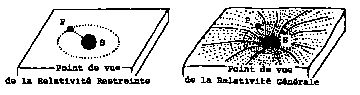
\includegraphics[width=0.5\linewidth]{figures/Fig02}
\end{center}
} % NB: \visible rend visible son argument, c'est-à-dire qu'il faut mettre ce 
  % qu'on veut rendre visible entre accolades par la suite contrairement à \onslide
  % qui joue le rôle d'une bascule.

\onslide<3->
Et le texte qui suit

\end{frame}

\begin{frame}[fragile]
\frametitle{Exemples}
\framesubtitle{Apparition d'une équation en plusieurs temps}

L'idée est d'utiliser \verb|\onslide| pour faire apparaître les morceaux uns à 
uns. Cela correspond à des bascules qui imposent le comportement de tout ce qui 
suit jusqu'au prochain \verb|\onslide|. Par exemple, avec votre vieil ami 
l'oscillateur harmonique

$$
\onslide<3>
	1\times
\onslide<2->
	\frac{\dd^2\theta}{\dd t^2} + 
\onslide<4>
	\overbrace{
\onslide<2-> 
	\frac{g}{\ell}
\onslide<4>
	}^{={\omega_0}^2}
\onslide<2-> 
	\times\theta
	=
\onslide<5>
	\overbrace{
\onslide<2-> 
	A
\onslide<5>
	}^{=\theta\e{éq}\times{\omega_0}^2}
\onslide<2-> 
$$

\onslide<6->
Le mieux est d'écrire l'équation voulue en une fois avec tous les rajouts et de découper ensuite. Par exemple ici, ce serait

\onslide<7->
$$
	1\times
	\frac{\dd^2\theta}{\dd t^2} + 
	\overbrace{  	\frac{g}{\ell}  	}^{={\omega_0}^2}
	\times\theta	=
	\overbrace{	A	}^{=\theta\e{éq}\times{\omega_0}^2}
$$


\end{frame}


\end{document}


